\documentclass[../main.tex]{subfiles}

\begin{document}

\subsection{강의 계획}
본 교재는 Python 3.7의 기본적인 문법을 익힐 수 있는 내용과 예제들이 수록되어 있습니다.
난이도는 프로그래밍 언어를 처음 접하더라도 익힐 수 있도록 구성되어 있으며, 상황에 맞추어 유동적으로 진행할 예정입니다.
본 수업은 algorithm알고리즘\footnote{간단히 말해서, 어떤 값들을 입력받아 값들을 출력하는 잘 정의된 과정을 말합니다.}을 배우는 것보다는 Python 3 언어의 기본적인 문법 숙지와 더불어 자주 사용되는 패턴에 익숙해지는 것에 초점을 맞추고 있습니다.
또한, 정보과학적인 사고(순차적으로 논리적인 비약이 없이 문제 해결을 할 수 있는 능력)를 배우고 간단한 알고리즈믹 문제의 해결법을 배우는 것이 목적입니다.
아래의 진도표는 회차 당 세 시간 수업을 기준으로 한 것으로, 가변적일 수 있습니다.

\begin{description}
  \item[1회차] Python 소개 및 기본 요소
  \item[2회차] Functions함수와 Conditionals조건문
  \item[3회차] Boolean Functions불리언 함수와 Loops반복문 기본
  \item[4회차] Lists리스트, Strings문자열, Counters카운터
  \item[5회차] Quantifiers한정자와 While 문
  \item[6회차] Loops반복문 응용과 파일 입출력
  \item[\sout{7회차}] \sout{Toy Robot}
  \item[7회차] 재귀법Recursion과 Python의 다양한 객체
  \item[8회차] 람다Lambda 함수
\end{description}

기본적으로 알고리즘보다는 언어 자체의 문법과 활용에 초점을 맞춘 커리큘럼이므로, 알고리즘을 본격적으로 다루기 위해서는 자료 구조와 알고리즘에 대해서 깊게 다루는 서적을 읽어보시는 것을 추천드립니다.
Python과 같이 언어를 익히고 난 다음에는 알고리즘을 배우고 실제로 구현할 수 있는 준비가 되어 있을 것입니다.

알고리즘에 대해서 더 배우고 싶으시다면 흔히 CLRS라고 불리우는 \textit{Introduction to Algorithms 3/e (MIT Press, 2009)}를 추천드립니다.
혹시 더 깊은 이해를 원하신다면, 저도 아직 읽어보지는 못했지만 커누스 교수의 TAOCP로 불리우는 \textit{The Art of Computer Programming} 시리즈\footnote{커누스 교수가 1968년부터 집필을 시작해 현재는 4권의 일부분까지 완성되어 있으며, 현재 7권까지 계획이 되어 있습니다. 빌 게이츠는 본인이 훌륭한 프로그래머라고 생각하면 TAOCP를 읽어보고, 다 읽을 수 있다면 자신에게 이력서를 보내라고 하였습니다. 여담으로, 커누스 교수는 이 책의 조판을 위해서 본 교재를 위해서 사용된 \TeX을 개발하였습니다.}를 읽어보시면 됩니다.

\subsection{들어가기 전에}
Python은 문법이 단순하면서도 활용 가능성이 무궁무진한 언어입니다.
단순히 `정보과학'만을 위해서 Python을 배운다기보다는, 평생 활용할 수 있는 도구를 배우는 것입니다.
Python은 R이나 Matlab 등과 함께 학문적인 용도로도 쓰임이 많은 언어입니다.
특히 Matlab과 다르게 Python은 오픈 소스에 무료인데다가, 단순히 데이터 처리만을 위한 언어가 아닙니다.
NumPy와 Matplotlib 등의 패키지를 활용한다면 Matlab이나 Mathematica와 같은 상용 프로그래밍 언어가 할 수 있는 다양한 작업들을 대등하게 할 수 있기도 합니다.

실제로 저는 학업 중 물리학, 천문학, 화학, 생물학 등의 분야에서 데이터 분석 및 차트 제작을 위해 Python을 활용하거나, Raspberry Pi와 연동하여 다양한 센서를 사용해 프로젝트를 진행하는데에도 사용했습니다.
또한 Django 등의 프레임워크를 사용한다면 웹서버를 구축할 수도 있는데, YouTube, Dropbox, Facebook, Netflix, Google, Instagram, Spotify 등의 유명 사이트들이 Python을 활용하여 서비스를 제공하고 있습니다.
이처럼 Python은 배워두면 무궁무진한 방면에서 활용할 수 있는 가능성을 가지고 있는 언어입니다.

\subsection{Python이란?}
\begin{figure}[htbp]
  \centering
  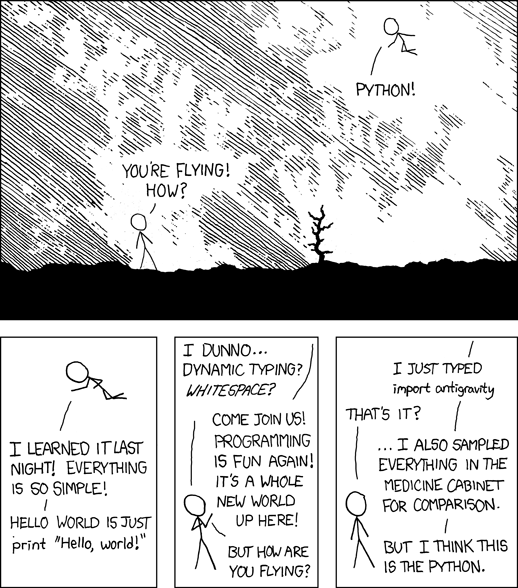
\includegraphics[width=0.6\linewidth]{./figures/xkcd_python}
  \caption*{흔히 Python을 ``batteries included''(배터리가 들어간) 언어라고 합니다.}\label{fig:meme}
\end{figure}
Python은 1991년에 Guido van Rossum이 발표한 프로그래밍 언어로, 문법이 굉장히 쉬우면서도 높은 생산성을 가지고 있는 언어입니다.\footnote{그가 1989년 크리스마스 연휴에 취미로 Python을 제작하였던 것이 그 시작입니다.}
특히 pseudocode의사코드와 유사하기 때문에 비교적 배우기 쉬워, 많은 학교에서 프로그래밍 입문 수업 언어로 Python을 채택하고 있습니다.
또, \textbf{프로그래밍 언어로 할 수 있을 법한 거의 모든 기능들이 이미 Python을 위한 패키지로 구현되어 있습니다.}
이 때문에 Python을 흔히 ``batteries included''라고 부릅니다.
따라서 속도가 중요한 작업이 아니라면 C/C++보다 Python을 쓰는 것이 효율적입니다.
(연산이 아니라 업무의 효율을 말하는 것입니다.)

프로그래밍에 익숙치 않더라도 컴퓨터에 관심이 많다면 C, C++, Java 등의 언어와 함께 Python도 한 번 쯤 들어보았을 정도로, Python은 점유율 상위 다섯 언어 안에 드는 주류 언어입니다.
Python은 1995년에 등장한 Java보다도 오래 전에 만들어진 언어로, 긴 역사를 가지고 있습니다.
그 만큼 버전의 숫자도 큰데, 이 글을 작성하는 현 시점에서 Python 2의 최신 버전은 2.7.16, Python 3의 최신 버전은 3.7.3입니다.
한동안은 Python 2와 Python 3가 동시에 개발되기도 하였고, Python 3보다는 Python 2를 사용하는 것이 낫다고 말하던 때가 있었습니다.\footnote{1, 2년 전까지만해도 Python 2 vs Python 3의 논쟁이 비일비재하게 일어났었습니다.}
그러나 현재는 Python 3를 배우고 사용하는 것이 권장됩니다.
Python 2는 2.7이 최종 버전이고, 이후에는 bugfix 릴리즈만 있을 예정인데다가 2020년까지만 지원을 할 예정입니다.
나아가 최신 버전의 Ubuntu(Linux 배포판의 한 버전)는 Python 3를 기본 Python 버전으로 설정하고 있습니다.

\textbf{Python은 interpreter인터프리터 언어입니다.}
Interpreter 언어란 소스 코드를 한 줄씩 기계어\footnote{기계가 바로 이해할 수 있는 저급 언어로, 0과 1의 이진수로만 구성되어 있는 언어로, 모든 CPU를 구동시키기 위해서는 C와 같은 고급 언어를 저급 언어로 변환시키는 과정이 필요합니다.}로 번역하는 방식의 언어입니다.
조금 더 가독성을 높인, 기계어와 일대일 대응이 되는 (마찬가지로 저급 언어인) 어셈블리어가 있기도 합니다.
고급 언어를 기계어로 변환시키는 방법은 크게 두 가지가 있습니다.
Compiler컴파일러와 interpreter입니다.
C와 같은 언어는 compiler 언어로, 코드 전체를 한꺼번에 기계어로 변환시킵니다.
이 때문에 실행 속도는 빠르다는 장점이 있지만, 코드를 수정하기 위해서는 다시 한 번 전체를 기계어로 변환시키는 과정이 필요합니다.
반면 Python은 한 줄씩 기계어로 번역하기 때문에 실행 속도는 다소 느리지만, debug디버그\footnote{코드에서 bug버그, 즉 오류를 제거하는 것을 의미합니다.}에 유리합니다.
한 줄씩 실행하기 때문에 애초에 compile을 거부하는 compiler 언어와는 다르게 버그가 있는 해당 줄까지 코드를 실행시켜주기 때문입니다.
이러한 장단점 때문에 프로그램의 골격을 Python으로 만들고, 빠른 연산이 필요한 부분만 C로 만드는 것도 가능합니다.

마지막으로, Python이 얼마나 쉽고 직관적인 언어인지 알아봅시다.
만약 A+가 F, C+, B0, A-, A+에 있으면 "A+가 있습니다."를 실행해주는 Python 코드를 봅시다.
\begin{minted}[mathescape,
               breaklines,
               numbersep=5pt,
               frame=lines,
               framesep=2mm]{python}
if "A+" in ["F", "C+", "B0", "A-", "A+"]: print("A+가 있습니다.")
\end{minted}
프로그래밍을 할 줄 모르더라도 저 코드를 이해할 수 있을 것입니다.
이처럼 Python은 인간이 사고하는 방식을 그대로 옮겨 놓았다고 해도 과언이 아닐만큼이나 직관적입니다.
익숙해진다면 자신이 하고 싶은 일을 코드로 옮기려고 끙끙댈 필요 없이, 생각하는 그대로 코드를 작성할 수 있을 것입니다.
참고로, 이와 같은 일을 하려면 C언어에서는 다음과 같이 해야 합니다.
\begin{minted}[mathescape,
               linenos,
               breaklines,
               numbersep=5pt,
               frame=lines,
               framesep=2mm]{c}
#include <stdio.h>
#include <string.h>
int main(void) {
    char grades[][3] = {"F", "C+", "B0", "A-", "A+"};
    for (int i = 0; i < 5; ++i) {
        if (strncmp(grades[i], "A+", 2) == 0) {
            printf("A+가 있습니다.\n");
        }
    }
    return 0;
}
\end{minted}
단 한 줄의 Python 코드로 될 일을 C 언어로는 10줄 이상으로 작성해야 하는 것입니다.

\subsection{Python의 기본 요소}
\subsubsection{Hello, World}

\begin{figure}[htpb]
  \centering
  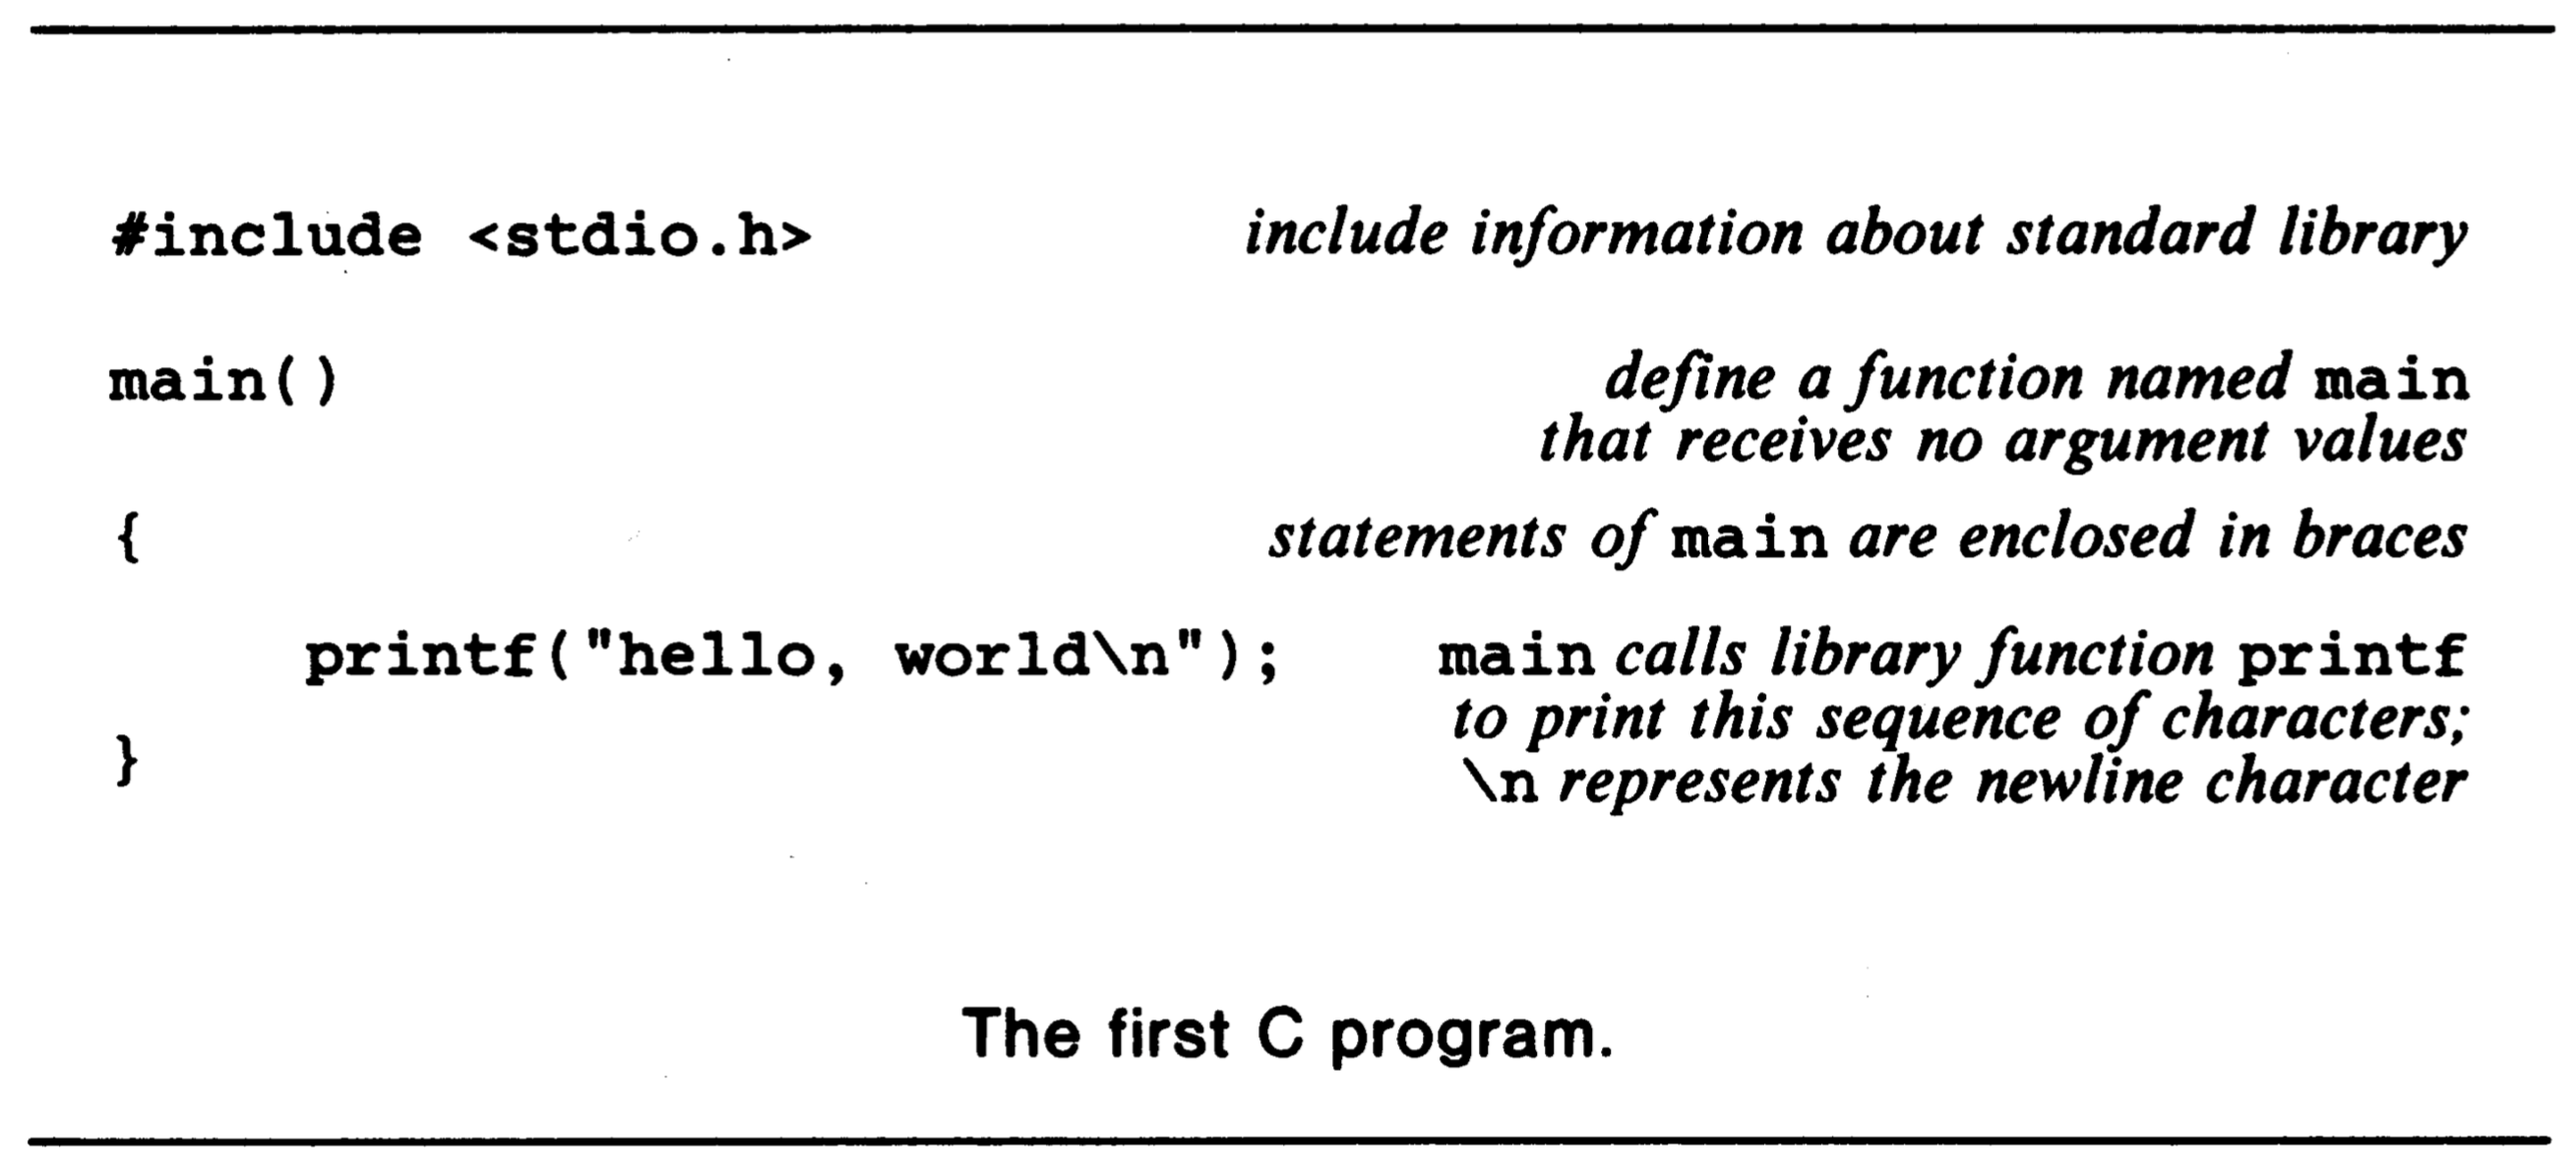
\includegraphics[width=0.8\linewidth]{./figures/hello_world.png}
  \caption*{K\&R \textit{The C Programming Language}의 첫 프로그램}
\end{figure}

1978년에 씌여진 K\&R이라고 불리우는 \textit{The C Programming Language}에서 예시로 사용된 이후 첫 프로그램은 보통 \texttt{Hello, World!}를 출력하는 것으로 시작됩니다.
먼저, IDE에 다음과 같은 코드를 입력해봅시다:
\begin{minted}[mathescape,
               linenos,
               breaklines,
               numbersep=5pt,
               frame=lines,
               framesep=2mm]{python}
print("Hello, World!")
\end{minted}
실행시켜보면 \texttt{Hello, World!}가 출력될 것입니다.
C 코드에서는 \texttt{include} 등 이것저것 따로 입력해야 할 것이 있는데, Python에서는 사뭇 간단한 것을 볼 수 있습니다.
이제 Python의 문법에 대해서 본격적으로 알아봅시다.

\subsubsection{Values값과 Variables변수}
윈도우를 쓴다면 명령 프롬프트나 powershell, 맥이나 리눅스와 같은 유닉스 계열을 쓴다면 터미널, 혹은 그냥 IDE에 내장된 쉘shell에 다음을 입력해 봅시다.
Interpreter 언어이기 때문에, 명령을 한 줄씩 입력하여 명령을 수행할 수 있습니다.
(\texttt{>>>}는 직접 입력하는 것이 아닙니다.)
\begin{minted}[mathescape,
               linenos,
               breaklines,
               numbersep=5pt,
               frame=lines,
               framesep=2mm]{python}
>>> a = (1+2+3+4)/2
>>> b = a - 1
>>> c = 3
>>> print(b + c)
7
>>> print(b, c)
4  3
>>> d = c
>>> a = d
>>> print(a)
3
\end{minted}
\texttt{a = (1+2+3+4)/2}는 등호 왼쪽에 있는 \texttt{a}에 등호 오른쪽에 있는 $\frac{1+2+3+4}{2}$를 배정한다는 뜻입니다.
즉, 수학에서 말하는 등호와는 의미가 다른 것이지요.
줄 2의 \texttt{b = a - 1}은 현재 \texttt{a}에 배정된 $\frac{1+2+3+4}{2} = 5$의 값에 1을 뺀 4를 \texttt{b}에 배정한다는 뜻입니다.
이 때, 좌변에 있는 \texttt{a}, \texttt{b	}, \texttt{c}를 variables변수\footnote{필요에 따라 영문의 `variable', 국문의 `변수'를 사용하여 서술하겠습니다. 이외의 용어도 처음에는 영문과 국문을 병기한 후, 필요에 따라 둘 중 하나의 표현만 사용하겠습니다.}, 우측의 \texttt{(1+2+3+4)/2}를 expression표현이라고 합니다.
또한 이러한 변수에 배정되는 것을 value값이라고 합니다.
다시 위의 예시로 돌아가서, 줄 2에 있는 좌변의 \texttt{b}는 variable, 우변의 \texttt{a - 1}는 value인 것이죠.
영어 문장으로 ``Let \{variable\} be \{value\}.''가 말이 되는지 대입하여 보면 쉽게 알 수 있습니다.
Variable과 value는 문자인지 숫자인지의 여부가 아니라 대입이 되는 대상인지 대입이 되어지는 대상인지의 여부가 결정짓습니다.
물론, variable이 value 그 자체가 될 수 있습니다.
줄 8의 예시와 같은 경우, 우변의 \texttt{c}는 variable이면서 \texttt{d}라는 variable에 대입되는 value입니다.
그렇다면, 아래와 같은 표현을 어떨까요?
\begin{minted}[mathescape,
               breaklines,
               numbersep=5pt,
               frame=lines,
               framesep=2mm]{python}
>>> 10 = a
\end{minted}
지금까지 잘 따라왔다면, value가 위치해야 할 좌변에 value인 literal\footnote{어떤 객체에 value를 부여할 수 있는 것입니다. \texttt{0}은 \texttt{int} literal, \texttt{"python"}은 \texttt{str} literal입니다. \texttt{int}, \texttt{str}이 무엇인지는 조금 뒤에 type형이라는 것을 배우면 알 수 있습니다.}이 위치해 잘못된 syntax구문이라는 것을 알 수 있습니다.
\texttt{SyntaxError: can't assign to literal}이라는 오류 log를 볼 수 있을 것입니다.
(여담이지만, 앞으로 수 없이 많은 오류 log를 볼 텐데, 이를 꼼꼼히 읽어보는 습관을 들입시다.
오류 log를 무시하고 디버깅하는 것은 마치 백사장에서 바늘을 찾는 것과도 같습니다.)
혹은, ``let 10 be a"라는 표현이 말이 되지 않는다는 것을 통해서도 직관적으로 잘못되었음을 파악할 수 있습니다.

이러한 변수는 여러 가지 종류가 있습니다.
이를 data type자료형, 혹은 간단히 type형이라고 합니다.
\texttt{-1}, \texttt{0}, \texttt{76} 등의 값은 \texttt{int}\footnote{정수라는 뜻의 integer에서 따온 명칭입니다. 단, 수학에서 3.0은 정수이지만 \texttt{3.0}은 \texttt{float} type입니다.} type, \texttt{3.14159}, \texttt{0.}, \texttt{6.626e-34}, \texttt{6.022E23} 등의 값은 \texttt{float}\footnote{부동 소수점 혹은 떠돌이 소수점이라는 뜻의 floating point에서 따온 명칭입니다. 실수가 아니라 근삿값이라는 의미에 더 가깝습니다.} type, \texttt{"Hello, world!"}, \texttt{\textquotesingle python\textquotesingle}, \texttt{""} 등의 값은 \texttt{str}\footnote{나열이라는 뜻의 string에서 따온 명칭입니다.} type입니다.
Type에 대해서는 조금 뒤에 더 자세히 살펴봅시다.

변수는 어떤 값이 배정된 것이라고 했는데, 이것을 assign되었다고 하며 값이 written되었다고도 표현할 수 있습니다.
이렇게 변수에 저장된 값은 read읽을 수 있는데, 첫 예시의 줄 2처럼 \texttt{a}에 저장된 값 \texttt{5}를 불러오는 것이 이에 해당합니다.
또한 줄 4의 \texttt{print}를 통해서도 값을 읽어올 수 있습니다.

변수는 서로 다른 값이 배정될 수 있습니다.
첫 예시에서 줄 9를 보면, \texttt{5}가 저장되었던 \texttt{a}에 \texttt{3}이 저장된 \texttt{d}의 value가 다시 \texttt{a}에 쓰여지는 것을 볼 수 있습니다.
줄 10에서 이 사실을 재확인할 수 있고요.
이와 같이 변수는 재활용될 수 있고, 이는 개수를 세거나(counting) 특정 사건을 기록하기 위해 flag 등으로 사용하는데 도움이 됩니다.
\begin{minted}[mathescape,
               linenos,
               breaklines,
               numbersep=5pt,
               frame=lines,
               framesep=2mm]{python}
>>> summ = 0
>>> summ = summ + 1
>>> summ = summ + 1
>>> print(summ)
2
\end{minted}
더 자세한 활용은 차차 Python을 익혀가면서 알아봅시다.

이 뿐만이 아니라, Python은 여러 변수에 여러 값을 한 번에 배정하는 것(multiple assignment)을 허용합니다.
나아가 \textbf{변수의 swapping을 매우 손쉽게 할 수 있습니다.}
이 둘을 다음 예시를 통해 함께 확인합시다.
\begin{minted}[mathescape,
               linenos,
               breaklines,
               numbersep=5pt,
               frame=lines,
               framesep=2mm]{python}
>>> a, b, c = 2, 7, 12
>>> a, b, c = b, c, a
>>> print(a, b, c)
7 12 2
>>> a, b = b % a, a
>>> print(a, b)
5 7
\end{minted}
Multiple assignment를 허용하지 않는 대다수의 언어에서는 임시 변수를 도입해야 합니다.
예컨대 줄 5의 경우 아래와 같은 방법을 사용해야 합니다.
\begin{minted}[mathescape,
               linenos,
               breaklines,
               numbersep=5pt,
               frame=lines,
               framesep=2mm]{python}
>>> tmp = a
>>> a = b % tmp
>>> b = tmp
\end{minted}
Python에서는 마치 하노이의 탑을 연상시키는 이러한 과정을 시행하지 않아도 됩니다.

마지막으로, 변수의 이름으로 정할 수 없는 특정 문자열이 있습니다.
Python이 내부적으로 사용하는 \texttt{int}, \texttt{str}, \texttt{if}, \texttt{else}, \texttt{for}, \texttt{range}, \dots 등이 이에 해당합니다.\footnote{\texttt{int} 등 type 명은 배정이 가능하지만, 형 변환을 위한 함수로 사용되므로 사용하면 안됩니다. 위에 나왔던 코드 중 \texttt{summ}이라고 썼던 변수명도 \texttt{sum}으로 쓰지 않은 이유는 \texttt{sum}에 해당하는 내장 함수가 있기 때문입니다.}
그리고 변수명은 영어 대소문자, 숫자, 그리고 \texttt{\_}로만 이뤄져 있어야 합니다.
(Python 3부터는 한글로도 이름을 명명할 수 있습니다.)
나아가 숫자로 시작할 수 없는데, \texttt{1st\_name}과 같은 문자열을 변수명으로 지정할 수 없는 것입니다.

\subsubsection{Expressions표현}
Expression은 variable, value, 그리고 operator들의 조합입니다.
우리가 흔히 부르는 사칙 연산 \texttt{+}, \texttt{-}, \texttt{*}, \texttt{/}와, 나머지를 구해주는 \texttt{\%}, 지수를 뜻하는 \texttt{**} 등이 이에 해당합니다.
\textbf{주의할 점은, \texttt{\^{}}이 지수를 뜻하는 것이 아니라 \texttt{**}이라 것입니다.}
또한 \texttt{//}는 몫을 구해줍니다.
아래의 예시를 봅시다.
\begin{minted}[mathescape,
               linenos,
               breaklines,
               numbersep=5pt,
               frame=lines,
               framesep=2mm]{python}
>>> 12 + 5
17
>>> 12 - 5
7
>>> 12 * 5
60
>>> 12 / 5
2.4
>>> 12 // 5
2
>>> 12 % 5
2
>>> 12 ** 5
248832
>>> 12 ^ 5
9
\end{minted}
\texttt{\^{}}는 bitwise XOR의 연산자로서, $12 = 1100_2$, $5 = (0)101_2$이므로 digit이 다른 $2^3, 2^2, 2^1$ 자릿수만 1을 취한 $1001_2 = 9$가 \texttt{12 \^{} 5}의 값입니다.
\texttt{\^{}}은 지수의 연산이 아닙니다!
연산의 순서는 기본적으로 괄호(\texttt{(\dots)}), unary 연산(\texttt{+x}, \texttt{-x}), 지수(\texttt{**}), 곱셈/나눗셈/나머지 연산(\texttt{*}, \texttt{/}, \texttt{\%}), 덧셈/뺄셈(\texttt{+}, \texttt{-})의 순서입니다.
헷갈리는 경우나 혼동을 불러올 수 있는 경우에는 \texttt{(\dots)}를 사용하여 순서를 명시할 수 있습니다.
또는 논리적인 블럭이 되는 경우 괄호를 사용하여 묶어주는 것이 권장됩니다.

참고로, Python 2에서는 나눗셈을 할 때 정수끼리 행하면 몫만이 구해집니다.
\texttt{12 / 5 = 2}와 같이 말입니다.
반면 \texttt{12.0 / 5 = 2.0}와 같이 제수나 피제수 중 하나라도 \texttt{float} 형이면 결과도 실제 \texttt{float}의 나눗셈의 결과로 나옵니다.
위와 같은 결과를 인터넷이나 서적에서 보신다면 Python 2 코드이므로 유의하시기 바랍니다.\footnote{또한 이 교재도 원래 Python 2 기준으로 쓰여져 있었는데, 이와 관련해 미처 수정되지 않은 부분이 있다면 알려주시기 바랍니다.}

코드를 작성할 때에는 특별한 경우를 제외하고는 가독성이 중요합니다.
예컨대, 중복되는 값이나 의미가 있는 값은 특정 변수에 저장하여 해당 변수를 통해 식을 표현하는 것이 바람직합니다.
아래의 예시를 봅시다.
\begin{minted}[mathescape,
               linenos,
               breaklines,
               numbersep=5pt,
               frame=lines,
               framesep=2mm]{python}
>>> S = ((3 + 4 + 5) * (-3 + 4 + 5) * (3 - 4 + 5) * (3 + 4 - 5))**0.5
>>> a, b, c = 3, 4, 5
>>> s = (a + b + c) / 2
>>> S = (s * (s - a) * (s - b) * (s - c))**0.5
\end{minted}
비록 줄 수는 늘어났지만, 줄 1의 표현보다는 줄 4의 표현이 가독성이 높을 뿐만이 아니라 더 일반적이어서 값을 바꾸기 위해서는 줄 2의 숫자 부분만 변경을 하면 된다.
반면 줄 1의 표현의 경우 \texttt{+}와 \texttt{-}의 부호 구분에서 실수를 할 수 있고 다른 값을 대입하기 위해서는 12 부분에 수정을 가해야 한다.

마지막으로 소개할 문법은 위에서 잠시 언급한 개수 세기 등에서 유용하게 쓸 수 있습니다.
변수 뒤에 산술 연산자(\texttt{+}, \texttt{-}, \texttt{*}, \texttt{/}, \texttt{\%}, \texttt{**}) 뒤에 바로 \texttt{=}를 붙인 후 수를 쓰는 syntax입니다.\footnote{\texttt{int}나 \texttt{float}형에서는 모든 산술 연산자를 쓸 수 있고, \texttt{str}형에 대해서는 정의가 되어 있는 \texttt{+}만 사용할 수 있습니다.}
\texttt{x += 1}과 같이 말입니다.
이는 해당 변수에 저장된 값에 등호 뒤에 쓰인 값을 더한다는 의미로, \texttt{x = x + 1}과 동일한 의미를 가지고 있습니다.
아래와 같이 응용할 수 있습니다.
\begin{minted}[mathescape,
               linenos,
               breaklines,
               numbersep=5pt,
               frame=lines,
               framesep=2mm]{python}
>>> x = 4
>>> x += 2
>>> x
6
>>> x -= 1
>>> x
5
>>> x *= 2
>>> x
10
>>> x /= 5
>>> x
2
>>> x %= 3
>>> x
2
>>> x **= 3
>>> x
8
\end{minted}
참고로, C/C++이나 Java와 같은 언어에는 \texttt{++}, \texttt{--}와 같이 쉽게 1을 더하거나 뺄 수 있는 연산자가 있습니다.
\texttt{a}가 3의 값을 가지고 있었을 때 \texttt{a++}를 하면 4가 되는 것이지요.
C++의 ++이 해당 연산자에서 따온 것입니다.
그러나 \texttt{a++}과 \texttt{++a}에 따라서 연산 후 결과는 같지만 실제 코드에서 사용되는 위치에 따라 수행 결과가 달라지는 등 버그의 원인이 되기 때문에 Python이나 모던 언어에서는 해당 연산자를 문법에 넣지 않는 추세입니다.

\subsubsection{Types형}
위에서 간단히 소개한 바 있는데, variable의 종류를 type형이라고 합니다.
현재로서는 지금까지 언급한 \texttt{int}(정수형), \texttt{float}(실수형), \texttt{str}(문자열) 세 가지 type만 알아두시면 됩니다.
지금까지는 숫자가 실수형임을 명시할 때 \texttt{3.}과 같이 온점을 찍어 표현하였는데, type conversion형 변환이라는 것을 사용하여도 됩니다.
\textbf{형 변환은 정수형과 실수형 간에서 자유롭게 가능하고, 문자열의 경우에는 그 자체가 수일 경우에만 변환이 가능합니다.}
\begin{minted}[mathescape,
               linenos,
               breaklines,
               numbersep=5pt,
               frame=lines,
               framesep=2mm]{python}
>>> x = 76
>>> x
76
>>> float(x)
76.0
>>> str(x)
'76'
>>> pi = 3.14
>>> pi
3.14
>>> int(pi)
3
>>> str(pi)
'3.14'
>>> s = "1"
>>> s
'1'
>>> int(s)
1
>>> float(s)
1.0
\end{minted}
위 예시를 통해 필요한 모든 경우를 파악하셨을 것입니다.
또한, \texttt{type($\cdot$)}를 통해 직접 type을 확인할 수 있습니다.
\begin{minted}[mathescape,
               linenos,
               breaklines,
               numbersep=5pt,
               frame=lines,
               framesep=2mm]{python}
>>> print(type(76))
<class 'int'>
>>> print(type(76.))
<class 'float'>
>>> print(type("76"))
<class 'str'>
\end{minted}

\subsubsection{Input/Output입출력}
지금까지는 Python shell에서만 명령을 실행했습니다.
그렇기 때문에 \texttt{a}에 담긴 값을 알기 위해서는 굳이 \texttt{print(a)}가 아니라 \texttt{a}를 치는 것 만으로도 충분했습니다.
하지만 여러 줄의 코드를 한꺼번에 작성하여 실행할 때에는 이런 방식의 접근이 불가능합니다.
또, 코드를 실행 중일 때 어떤 입력을 받기 위해서는 지금까지와는 다른 방법이 필요합니다.
Shell과는 다르게 한 줄씩 직접 입력하는 방식이 아니기 때문입니다.
값을 출력하는 것은 지금까지 해왔던 것처럼 \texttt{print}를 사용하면 되는데, 아래에서 \texttt{print}에 대해 좀 더 알아보겠습니다.
Shell이 아니라 파일을 만들어서 실행시킵니다.
\begin{minted}[mathescape,
               linenos,
               breaklines,
               numbersep=5pt,
               frame=lines,
               framesep=2mm]{python}
today = "Monday"

print("Today is", today)
print("Today is " + today)

print("\nprintf style:")
print("Today is %s" % today)
print("Today is %(day)s" % {"day": today})

print("\nPython 3, back-ported to Python 2:")
print("Today is {}".format(today))
print("Today is {day}".format(day=today))

print("\nPython 3.6+, Formatted String Literals:")
print(f"Today is {today}")
\end{minted}
위 예시는 Python에서 \texttt{Today is Monday}를 출력하는 여러가지 방법을 나열한 것입니다.
첫 번째(줄 3)는 ,를 사용하여 \texttt{print} 함수 내의 여러 인자들을 출력하는 방식입니다.
자동으로 띄어쓰기가 들어간다는 것에 유의합니다.
두 번째(줄 4)는 문자열의 덧셈을 통해 출력한 것으로, 띄어쓰기는 직접 앞 \texttt{Today is}에 추가하였습니다.
다음 예시부터는 문자열 포맷팅에 관한 내용입니다.
먼저 줄 7과 8의 예시는 과거 사용되었던 방식으로, 현재에도 사용할 수 있는 방식입니다.
C 언어의 \texttt{printf}와 유사한 방식입니다.
\texttt{\%s}는 뒤 \texttt{\%} 뒤의 변수를 문자열 형식으로 넣으라는 뜻입니다.
만약 이름을 붙여서 지정하고 싶다면 줄 8과 같이 사용하면 됩니다.
Python 3에서 시작되어 현재는 Python 2로 백포트된 문자열 포맷팅 방식은 줄 11과 12에 나와 있습니다.
\texttt{\{\}}로 지정된 부분에 뒤 \texttt{.format()} 메소드 내부의 인자가 대입되는 것을 확인할 수 있습니다.
마지막 15 줄의 방식이 가장 최근에 도입된 Formatted String Literals라는 것입니다.
문자열 앞에 \texttt{f}를 붙인 후 단순히 중괄호 안에 원하는 변수 이름을 넣으면 대입이 됩니다.
만약 Python 3.6 이상 버전을 쓰고 있다면 사용이 가능하므로 되도록이면 해당 방식을 사용하는 것이 권장됩니다.

이제는 값을 입력하는 법에 대해 알아봅시다.
\texttt{input($\cdot$)} 함수를 사용하면 됩니다.
다음과 같은 예시를 살펴봅시다.
\begin{minted}[mathescape,
               linenos,
               breaklines,
               numbersep=5pt,
               frame=lines,
               framesep=2mm]{python}
today = input("What day is it today? ")
print("Today is", today)

s = input("Enter the number you want to know the square root of: ")
n = float(s)
print(n**.5)
\end{minted}
위 코드를 실행시키면 창에 \texttt{What day is it today? }가 출력된 후 입력이 될 때까지 기다립니다.
키보드로 값을 입력한 후--\texttt{Thursday}를 입력했다고 합시다--리턴 키를 치면 값이 입력되고, \texttt{Today is Thursday.}가 출력될 것입니다.
또한, 수를 입력 받을시 \texttt{int($\cdot$)}나 \texttt{float($\cdot$)}로 형 변환을 수행해줘야 합니다.
\textbf{\texttt{input($\cdot$)}이 넘겨주는 값은 항상 \texttt{str} 형이기 때문입니다.}

\subsection{예제}
\begin{enumerate}
  \item 1부터 $n$까지 자연수의 제곱의 합과 세제곱의 합의 차이를 구하는 코드를
    작성하세요.
    단, 아직 배우지 않은 \verb|for| 문 없이 다음의 공식을 사용하세요:
    \begin{align*}
      \sum^{n}_{k = 1} k^2 &= \frac{n(n + 1)(2n + 1)}{6}\\
      \sum^{n}_{k = 1} k^3 &= \left(\frac{n(n + 1)}{2}\right)^2
    \end{align*}
    \begin{minted}[mathescape,
                   linenos,
                   breaklines,
                   numbersep=5pt,
                   frame=lines,
                   framesep=2mm]{python}
n = int(input("Enter n: "))
# Add here!
    \end{minted}

  \item 원탁 주위에 \verb|a|, \verb|b|, \verb|c|, \verb|d|, \verb|e|가 앉아
    있습니다.
    각자는 자신이 좋아하는 정수를 종이에 적은 후, 양 옆에 앉은 사람의 정수를
    더합니다.
    최종적으로 각자가 얻게된 수를 출력하도록 다음 코드를 완성하세요:
    \begin{minted}[mathescape,
                   linenos,
                   breaklines,
                   numbersep=5pt,
                   frame=lines,
                   framesep=2mm]{python}
a = int(input("Enter a: "))
b = int(input("Enter b: "))
c = int(input("Enter c: "))
d = int(input("Enter d: "))
e = int(input("Enter e: "))
print("Favorite integers: ", a, b, c, d, e)
# Add here!
print("Final integers: ", a, b, c, d, e)
    \end{minted}

  \item 이차방정식 $\verb|a|x^2 + \verb|b|x + \verb|c| = 0$의 해를 구하는
    코드를 작성하세요.
    단, 판별식 $\verb|b|^2 - 4\verb|ac| > 0$이라고 가정합니다.

    \begin{minted}[mathescape,
                   linenos,
                   breaklines,
                   numbersep=5pt,
                   frame=lines,
                   framesep=2mm]{python}
a = int(input("Enter a: "))
b = int(input("Enter b: "))
c = int(input("Enter c: "))
# Add here!
# x1 = ...
# x2 = ...
print("Solutions for the quadratic equation are ", x1, " and ", x2)
    \end{minted}

  \item 다음 표현의 값을 예상하세요.
    \begin{minted}[mathescape,
               linenos,
               breaklines,
               numbersep=5pt,
               frame=lines,
               framesep=2mm]{python}
>>> 3*2**6+12
???
>>> 32/7+2**3/3
???
>>> 13/3%3+2.0
???
>>> 13//2/4.
???
>>> int(2**(1/2))+1
???
    \end{minted}

  \item Python 3에서 가능한 변수명을 모두 고르세요.
    \begin{itemize}
      \item \texttt{if}
      \item \texttt{sum}
      \item \texttt{max}
      \item \texttt{1st\_var}
      \item \texttt{var\_1}
      \item \texttt{this+that}
      \item \texttt{\_self}
      \item \texttt{변수}
      \item \texttt{r\&e}
    \end{itemize}

  \item 다음 코드는 여섯 개의 실수 \verb|x1|, \verb|x2|, \verb|x3|, \verb|y1|,
    \verb|y2|, \verb|y3|을 입력받습니다.
    \verb|i|가 \verb|1|, \verb|2|, \verb|3|을 취할 때 $(\verb|xi|,
    \verb|yi|)$가 좌표평면에서 서로 다른 세 점을 나타내는 좌표라고 가정합니다.
    이때 세 점이 이루는 삼각형의 면적을 계산하는 코드를 작성하세요.\\
    참고로,
    \begin{itemize}
      \small
      \item 세 변의 길이가 $a$, $b$, $c$인 삼각형의 면적은 $s = \frac{a + b +
        c}{2}$일 때 $\sqrt{s(s - a)(s - b)(s - c)}$입니다.
      \item 또한, 어떤 두 벡터 $\vec{u}$와 $\vec{v}$가 이루는 삼각형의 면적은
        $\frac12 \norm{\vec{u} \times \vec{v}} = \frac12 \norm{\vec{u}}
        \norm{\vec{v}} \cos \theta$입니다.
      \item 이때, $\cos \theta = \frac{\vec{u} \cdot \vec{v}}{\norm{\vec{v}}
    \norm{\vec{u}}}$입니다.
    \end{itemize}
    \begin{minted}[mathescape,
                   linenos,
                   breaklines,
                   numbersep=5pt,
                   frame=lines,
                   framesep=2mm]{python}
x1 = int(input("Enter x1: "))
y1 = int(input("Enter y1: "))
x2 = int(input("Enter x2: "))
y2 = int(input("Enter y2: "))
x3 = int(input("Enter x3: "))
y3 = int(input("Enter y3: "))
# Add here!
# area = ...
print("Area of the triangle is", area)
    \end{minted}

  \item \verb|a|를 \verb|b|로 나눈 나머지를 \verb|%| 없이 사칙연산과 \verb|//|
  만으로 구하세요.
    \begin{minted}[mathescape,
               linenos,
               breaklines,
               numbersep=5pt,
               frame=lines,
               framesep=2mm]{python}
a = int(input("Enter a:"))
b = int(input("Enter b:"))
# Add here!
# r = ...
print("Remainder is", r)
    \end{minted}

  \item[참고.] 다음 코드는 양의 실수에 대해 올림 함수 $\lceil x \rceil = \min
    \{n \in \mathbb{Z} \mid n \geq x\}$를 계산합니다.
    \verb|int(·)|, \verb|+|, \verb|-|만을 사용하여 구현하세요.\footnote{정답:
    \raisebox{\depth}{\rotatebox{180}{\texttt{int(x - int(x) - 1) + int(x) + 1}}}}
    \begin{itemize}
      \item 힌트: \verb|int(·)| 함수의 그래프를 그려보세요.
    \end{itemize}
    \begin{minted}[mathescape,
                   linenos,
                   breaklines,
                   numbersep=5pt,
                   frame=lines,
                   framesep=2mm]{python}
x = float(input("Enter x:"))
# Add here!
# ceil_x = ...
print("Ceil(x) =", ceil_x)
    \end{minted}
\end{enumerate}
\end{document}
